\section{Les commandes de vol}
	\subsection{Les axes}
	Un aéronef peut bouger sur 3 axes :
	\begin{itemize}
		\item l'axe du roulis \anglais{roll} : il s'agit de l'axe gauche-droite. Cet axe se pilote via les ailerons qui sont actionnés via des mouvements latéraux du manche.
		\item l'axe du tangage \anglais{pitch} : il s'agit de l'axe avant arrière. Cet axe se pilote grâce à la gouverne de profondeur, actionnée via les mouvements longitudinaux du manche. 
		\item l'axe du lacet \anglais{yaw} : il s'agit de l'axe latéral. Cet axe se pilote grâce au gouvernail, actionné grâce aux palonniers.
	\end{itemize}
	
	\begin{figure}[H]
  		\centering
    		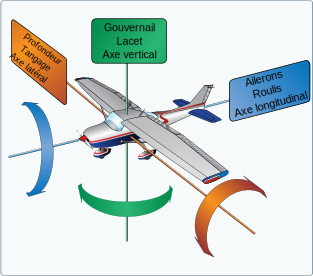
\includegraphics[width=0.6\textwidth]{01-EtudeAeronefs/img/axes.pdf}
  		\legende{Les 3 axes d'un aéronef}{img:axes}
	\end{figure}	
	
	\histoire{On doit à Robert Esnault-Pelterie, ingénieur français, l'invention des ailerons (1905) et du manche à balai (1906). Auparavant, les concepteurs d'avions utilisaient le gauchissement, c'est à dire la flexion de l'extrémité des ailes, pour assurer le contrôle latéral de leur aéronef.}
	
	\subsection{Contrôle en roulis}
	Le pilotage en roulis est principalement réalisé grâce à une action sur les ailerons.
	
	Lorsque le pilote actionne le manche d'un côté, l'aileron de l'aile du côté où le manche est incliné monte, tandis que l'aileron opposé descend. Cela provoque une dissymétrie de portance : la portance augmente du côté où l'aileron est baissé (même principe qu'un volet), tandis que la portance sur l'aile opposée diminue. En conséquence l'aile avec le surplus de portance monte et l'aile opposée descend.
	
	\begin{figure}[H]
  		\centering
    		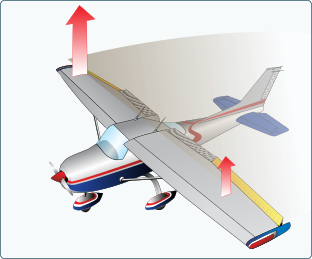
\includegraphics[width=0.6\textwidth]{01-EtudeAeronefs/img/virage.pdf}
  		\legende{Principe de mise en virage par action sur les ailerons}{img:virage}
	\end{figure}	
	
	\subsubsection{Le lacet inverse}
		Le lacet inverse est un effet secondaire (également parfois dit indésirable) du braquage des ailerons. Comme vu dans le chapitre \ref{chap:aero:trainee} \nameref{chap:aero:trainee}, une augmentation de la portance est toujours associée à une augmentation de la traînée. L'aile extérieure au virage aura donc tendance à freiner plus que l'aile intérieure. Par conséquence, le nez de l'avion aura tendance à pointer vers l'extérieur du virage. C'est ce que l'on appelle le lacet inverse.
		\begin{figure}[H]
			\centering
  			\includegraphics[width=0.6\textwidth]{01-EtudeAeronefs/img/lacetInverse.pdf}
  			\legende{Lacet inverse (à droite pour un virage à gauche)}{img:lacetInverse}	
		\end{figure}	
		
		Lors d'un virage, le pilote doit donc contrer ce lacet par une action adaptée au palonnier. Cette action s'appelle la conjugaison des commandes. Le pilote peut contrôler symétrie du virage grâce à la bille-aiguille (cf \ref{chap:etudeAer:indicateurVirage} \nameref{chap:etudeAer:indicateurVirage}).
	
	\subsection{Contrôle en tangage}
	Le contrôle en tangage est assuré par la gouverne de profondeur.

	La gouverne de profondeur est une surface \textbf{déportante}, c'est-à-dire qu'elle produit une force inverse en direction inverse des ailes (donc une force orientée vers le bas).
		\begin{figure}[H]
			\centering
  			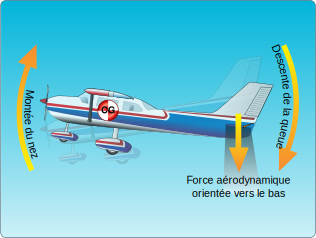
\includegraphics[width=0.6\textwidth]{01-EtudeAeronefs/img/gouverneProfondeur.pdf}
  			\legende{Commande de profondeur}{img:gouverneProfondeur}	
		\end{figure}
		
	\subsection{Le contrôle en lacet}
	Le contrôle en lacet est assuré par la gouverne de direction (également parfois appelé gouvernail). Cette gouverne, généralement située sur la queue de l'appareil, est une surface verticale que le pilote peut contrôler par une action sur le palonnier.
		\begin{figure}[H]
			\centering
  			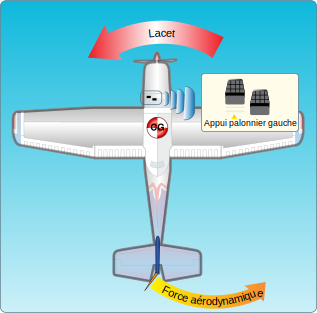
\includegraphics[width=0.6\textwidth]{01-EtudeAeronefs/img/gouverneDeDirection.pdf}
  			\legende{Commande de direction}{img:gouverneDeDirection}	
		\end{figure}	
		
		Quand le pilote appuie sur le palonnier, la gouverne de direction se braque du côté de l'appui. L'air vient alors taper dans la gouverne et provoque la rotation de l'appareil, le nez de l'avion se dirigeant du côté du palonnier appuyé. \\
		
		Cette gouverne est utilisée en virage pour coordonner le virage, et également à l'atterrissage par vent de travers, pour "décraber" (aligner l'axe de l'avion avec celui de la piste) au moment de l'impact de roues.
		
		Sur la plupart des avions, le palonnier sert aussi à diriger l'avion au sol.
		
		\subsubsection{Le roulis induit}
		Le roulis induit (sous entendu par le lacet) est un phénomène qui provoque l'inclinaison de l'avion lorsque le pilote effectue une action sur gouverne de direction (mise en dérapage).
		
		Si le pilote agit sur la gouverne de direction, il va mettre l'avion "en crabe". La portance sur l'aile du côté de l'action du pilote sera réduite, ce qui provoquera son enfoncement, et donc l'inclinaison de l'avion du côté de cette aile.
		
	\subsection{Systèmes de commande de vol}
		\subsubsection{Commandes mécaniques}
		Sur un avion léger, la vitesse faible et la surface limitée des gouvernes, sont actionnables par la seule force du pilote. Pour cela, le manche et le palonnier sont connectés aux gouvernes par un jeu de câble, de poulies de renvoi et de timoneries rigides.
		\begin{figure}[H]
		\centering
  			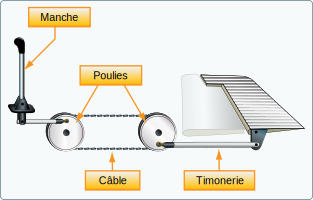
\includegraphics[width=0.6\textwidth]{01-EtudeAeronefs/img/cdvMecaniques.pdf}
  			\legende{Commande de vol mécaniques}{img:cdvMecaniques}	
		\end{figure}	
		
		\subsubsection{Commandes hydrauliques}
		Quand un aéronef devient plus lourd et plus rapide, on augmente la taille des gouvernes pour les rendre plus efficaces. Cette augmentation du flux d'air et la surface plus grande ont une conséquence : les gouvernes deviennent de plus en plus difficiles à man\oe uvrer, jusqu'à un point où il devient très difficile voire impossible de les faire bouger avec la seule force musculaire des pilotes.
		
		On a donc recours à des systèmes d'assistance hydrauliques. Grâce à de l'huile hydraulique mise en pression grâce à des pompes, des cylindres hydrauliques multiplient la force des pilotes.
		\begin{figure}[H]
		\centering
  			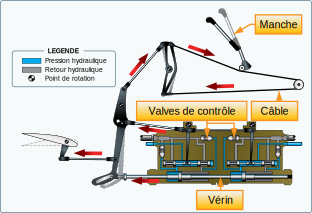
\includegraphics[width=0.55\textwidth]{01-EtudeAeronefs/img/cdvHydrauliques.pdf}
  			\legende{Commande de vol hydrauliques}{img:cdvHydrauliques}	
		\end{figure}	
		Dans ce type de commandes de vol, le manche reste physiquement connecté aux gouvernes de l'avion : en cas de panne du système hydraulique, l'avion reste pilotable, mais cela peut nécessiter une force considérable, voire que les 2 pilotes agissent ensemble sur les commandes.	
		
		Ce type de commande de vol se trouve typiquement sur les avions de ligne du constructeur Boeing.
		
		\subsubsection{Commandes de vol électriques}
		Désormais, certains constructeurs ont recours à des commandes de vol dites électriques \anglais{fly-by-wire}. Avec ce type de commande de vol, il n'existe plus aucun lien physique entre les commandes de vol et les gouvernes. Les ordres au manche des pilotes sont convertis en signaux électriques qui sont ensuite traités par des calculateurs (ordinateurs). Ceux-ci déterminent les valeurs de positions des gouvernes qui sont alors actionnées par des vérins hydrauliques.
		
		\histoire{Le premier avion de ligne commercial à utiliser des commandes de vol électriques est le Concorde, qui a effectué son premier vol en 1969. \\ En 1984, Airbus effectue le premier vol de l'A320, premier avion de ligne à commandes de vol numériques.}
		
		\info{La totalité de la flotte d'Airbus (sauf A300 et A310) dispose de commandes de vol numériques.}
		
		Les commandes de vol électriques permettent notamment de protéger le domaine de vol de l'avion. Il est par exemple pratiquement impossible de faire décrocher un Airbus : si le pilote agit sur le manche et approche l'incidence de décrochage, le calculateur empêchera la transmission de l'ordre vers les gouvernes. De même, les commandes de vol électriques peuvent protéger l'avion en terme de facteur de charge, de survitesse ou encore d'inclinaison.
		
		\subsection{Commandes de vol secondaires}
		Les dispositifs hyper et hyposustentateurs sont également considérés comme des commandes de vol, dites secondaires. Voir \ref{chap:aero:hyperHypoSutentateurs} \nameref{chap:aero:hyperHypoSutentateurs}.